\documentclass[a4paper]{article}
\usepackage[warn]{mathtext}
\usepackage[T2A]{fontenc}
\usepackage[utf8]{inputenc}
\usepackage[russian,english]{babel}
\usepackage{amsfonts}
\DeclareSymbolFont{T2Aletters}{T2A}{cmr}{m}{it}
\usepackage{caption} % подписи к рисункам в русской типографской традиции
\usepackage{graphicx}
\graphicspath{{graphs/}}
\DeclareGraphicsExtensions{.png}

\usepackage{xcolor}
\usepackage{hyperref}

\definecolor{linkcolor}{HTML}{0645AD} % цвет ссылок
\definecolor{urlcolor}{HTML}{0645AD} % цвет гиперссылок
 
\hypersetup{pdfstartview=FitH,  linkcolor=linkcolor,urlcolor=urlcolor, colorlinks=true}

\begin{document} % начало документа
 
\begin{center}
{Работа 2.2.1}\\
\large{Исследование взаимной диффузии газов}\\ 
\end{center} 

\section{Основные теоретические сведения}
Основные теоретические сведения о работе представлены в презентации (приложение 1).

\section{Обработка результатов}
По полученным в результате работы данным построим \hyperref[gr1]{график 1} зависимости U, которое при малом отношении добавочного газа к основному пропорционален разности теплопроводностей, от t.

\begin{figure}[h!]
\center{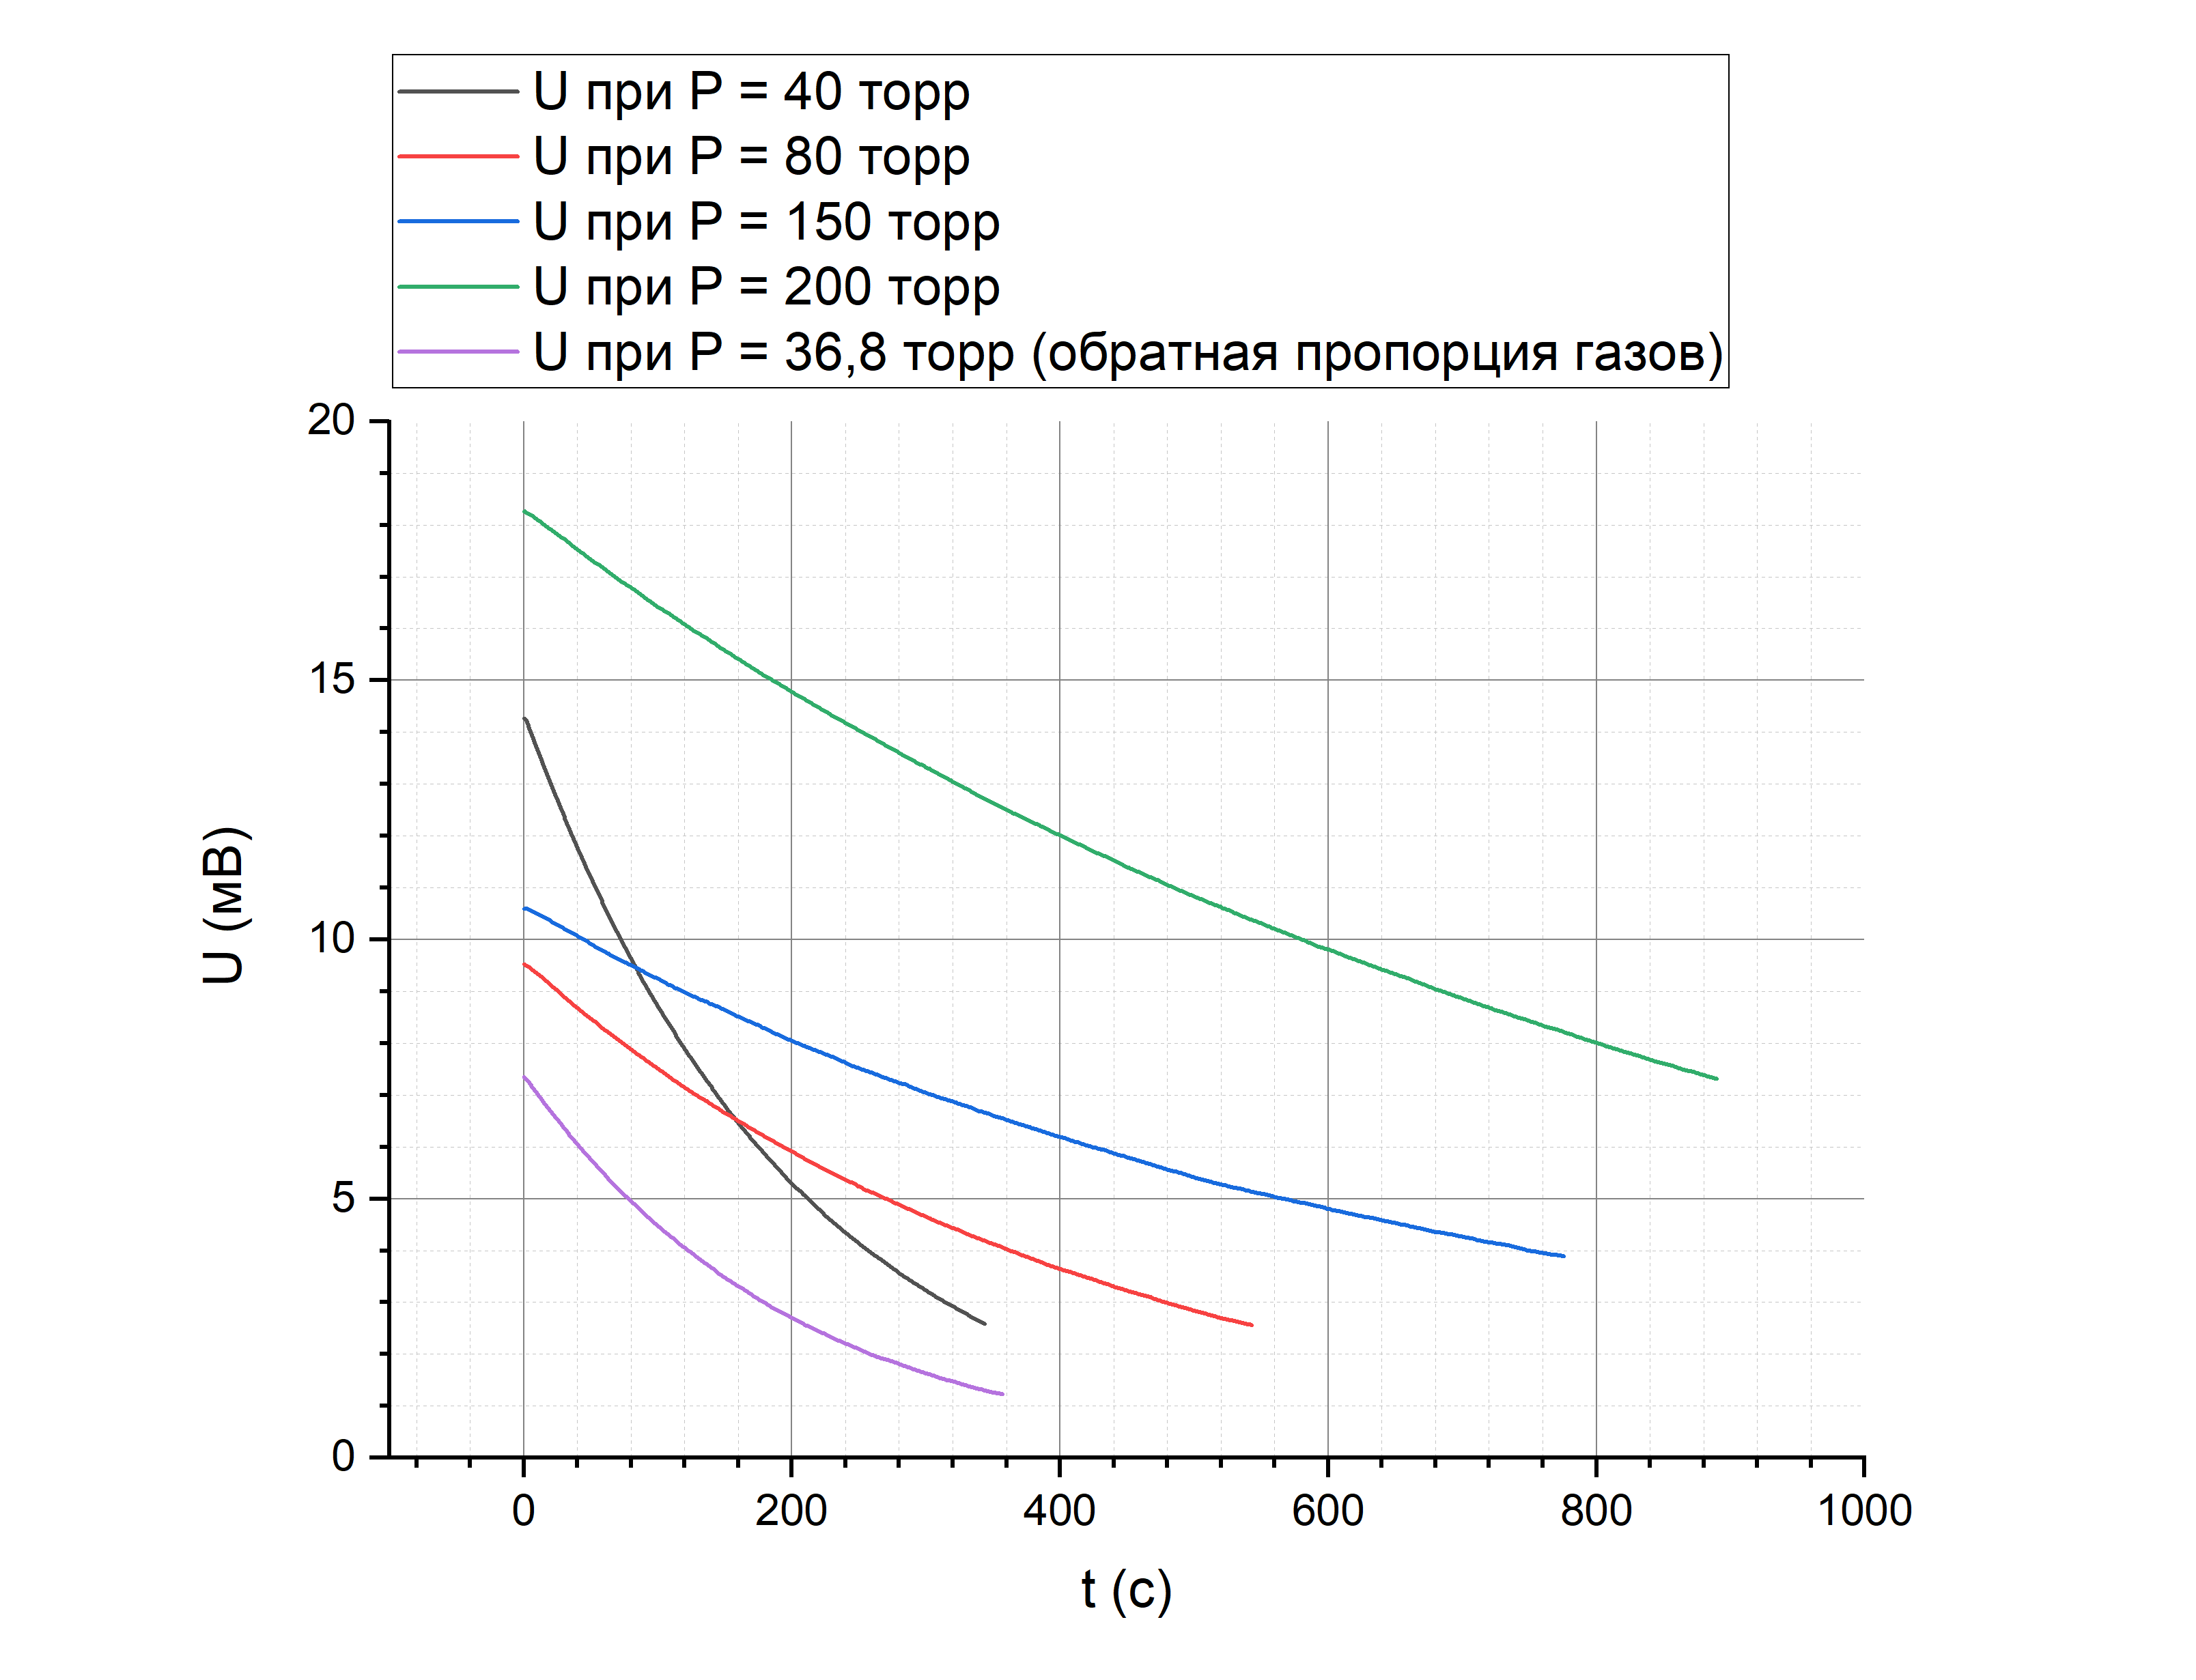
\includegraphics[width=\textwidth]{graph1}}
\caption*{График 1}
\label{gr1}
\end{figure}

\clearpage
Построим \hyperref[gr2]{график 2}, являющий собой ту же зависимость, но в логарифмическом масштабе.

\begin{figure}[h!]
\center{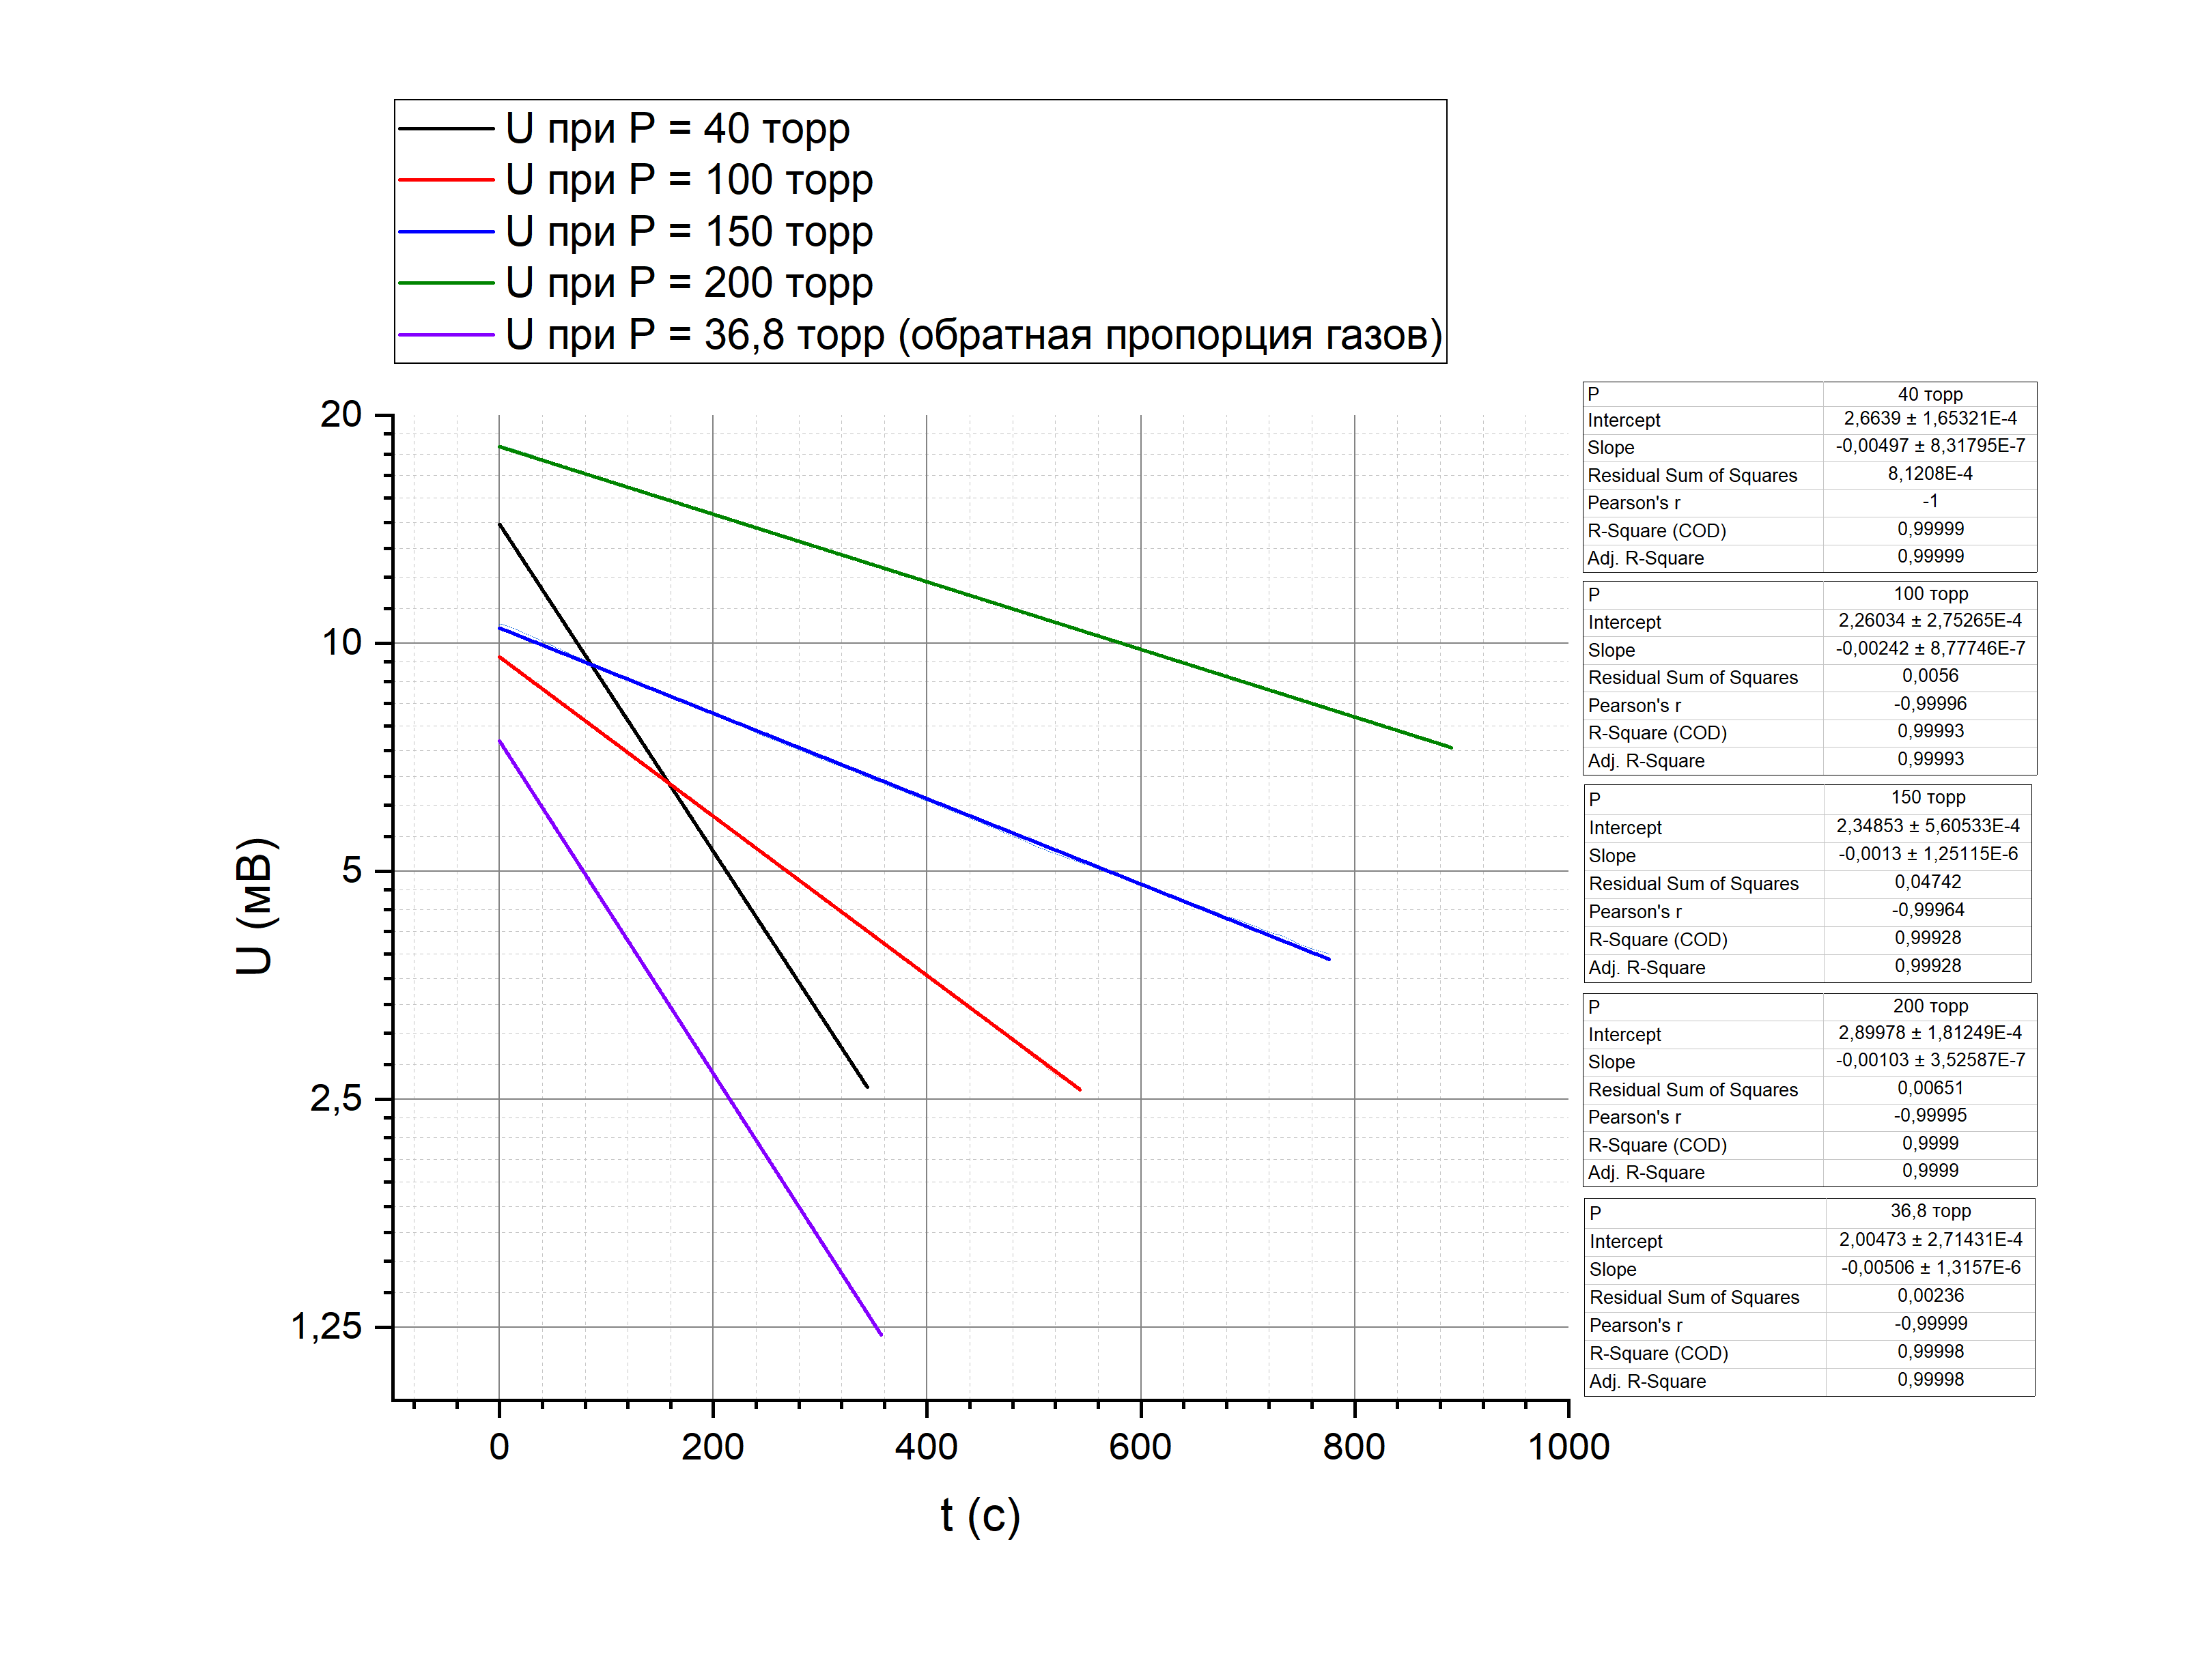
\includegraphics[width=\textwidth]{graph2}}
\caption*{График 2}
\label{gr2}
\end{figure}

По данным наклона полученных с помощью линейной аппроксимации данных, представленных на \hyperref[gr2]{графике 2}, получим значение коэффициента взаимной диффузии по \hyperref[frl]{формуле}
\begin{equation}\label{frl} 
D = Slope \cdot \frac{VL}{2S}
\end{equation} 
Полученные значения внесем в \hyperref[tb1]{таблицу 1}.

\begin{table}[h]
\centering
\caption*{Таблица 1}
\begin{tabular}{|l|l|l|}
\hline
\label{tb1}

P, торр & D, см$^2 /$c & $\sigma_D$, см$^2 /$c \\ \hline
40 & 9,4 & 0,2 \\ \hline
100 & 4,6 & 0,1 \\ \hline
150 & 2,46 & 0,06 \\ \hline
200 & 1,95 & 0,05 \\ \hline
36,8 (Обратное соотношение газов) & 9,6 & 0,3 \\ \hline

\end{tabular}
\end{table}

\clearpage
По данным \hyperref[tb1]{таблицы 1} построим \hyperref[gr3]{график 3} -- зависимость $D$ от $\frac{1}{P}$.

\begin{figure}[h!]
\center{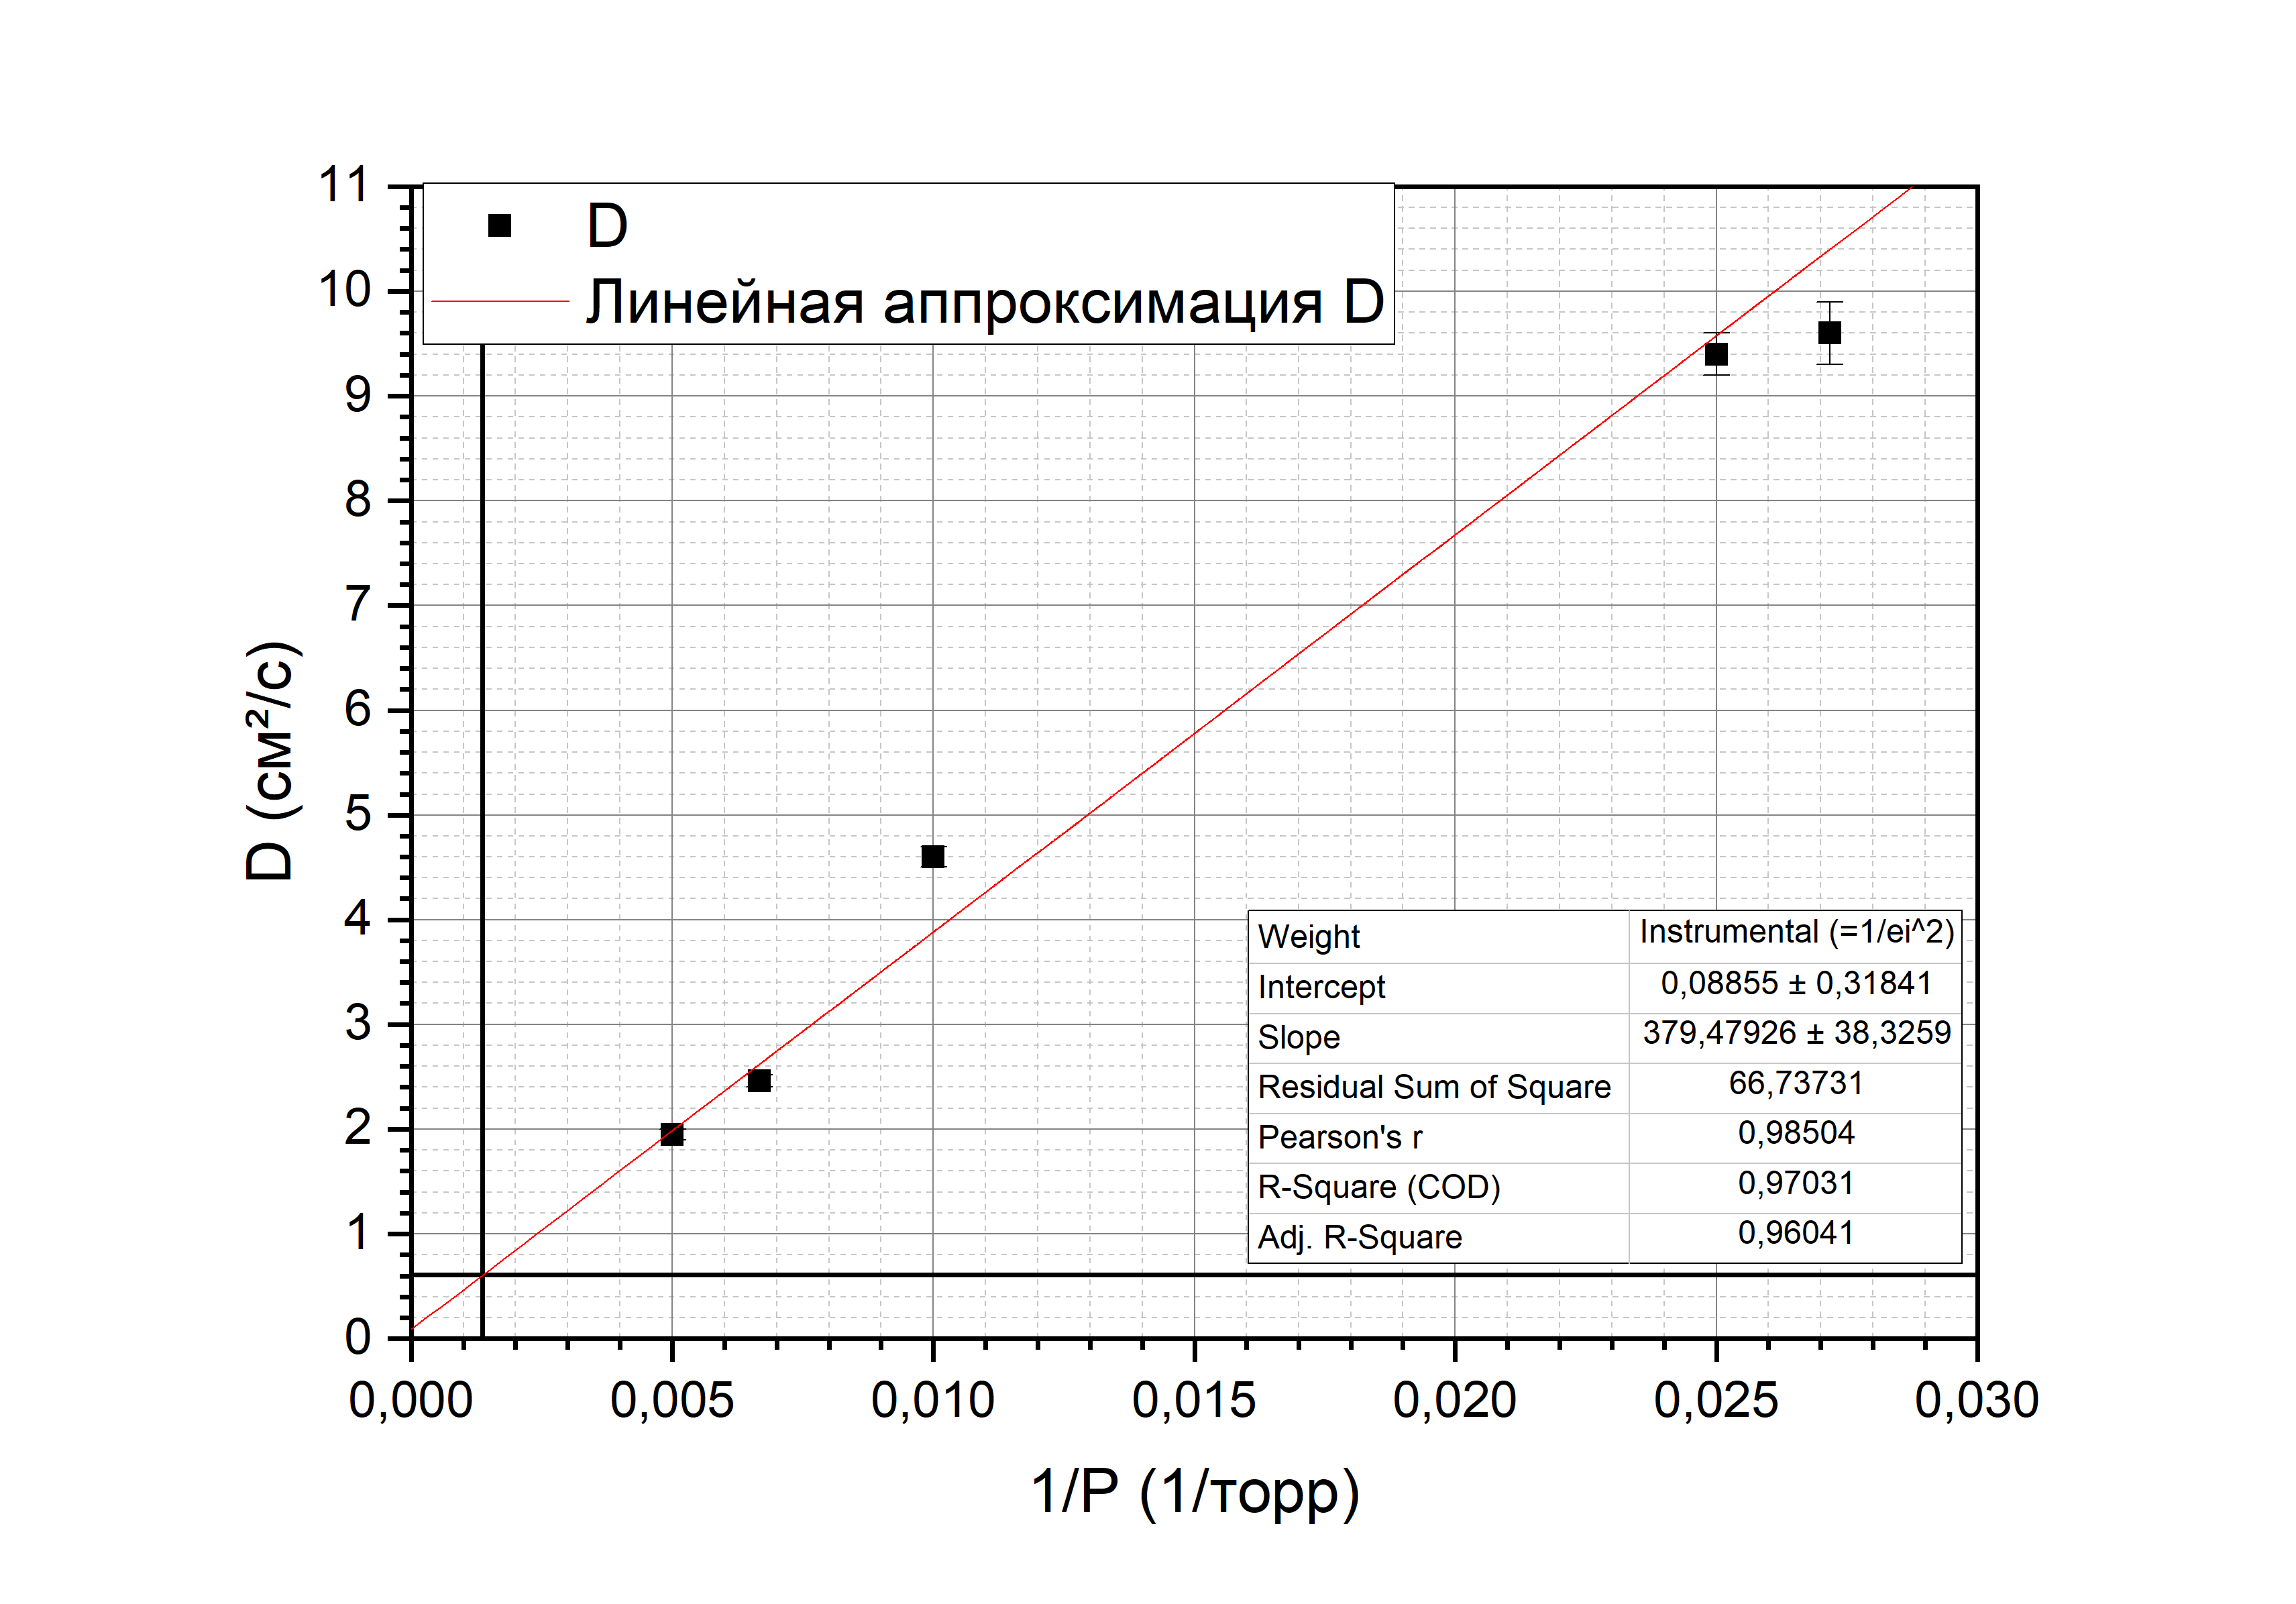
\includegraphics[width=\textwidth]{graph3}}
\caption*{График 3}
\label{gr3}
\end{figure}

По \hyperref[gr3]{графику 3} определим значение коэффициента взаимной диффузии при атмосферном давлении $P_0 = 730$ торр (данные на 28.02.2020 для г.~Долгопрудный). $D_0 = (0,60 \pm 0,05)$ см$^2 /$c

\section{Итоговый результат}
При атмосферном давлении значение коэффициента взаимной диффузии составило $(0,60 \pm 0,05)$ см$^2 /$c. Табличное значение при температуре $0^\circ C$ составляет $D_{table} = 0,62$ см$^2 /$c.

Длина свободного пробега гелия в воздухе при комнатной температуре составила $\lambda = (1,4 \pm 0,1) \cdot 10^{-7}$м.

Эффективное сечение столкнокения атомов гелия с молекулами воздуха составило $\sigma = (2,8 \pm 0,2) \cdot 10^{-19}$м$^2$.




\section{Вывод}
Таким образом, на практике проверен закон (8). Получено значение коэффициента взаимной диффузии при атмосферном давлении. Полученные данные сходятся с табличными. Также на практике проверено, что не имеет значение, какой из газов является примесью.




\end{document}
